%%%%%%%%%%%%%%%%%%%%%%%%%%%%%%%%%%%%%%%%%%%%%%%%%%%%%%%%%%%%%%%%%%%%%%%%%%%%%%%%
\section{Methods}
\subsection{Problem Formulation}
The perceptive traversal task is formalized as a goal-conditioned Partially Observable Markov Decision Process (POMDP). At each time step $t$, the policy $\pi_\theta$ receives a partial observation $\mathbf{o}_t$ encapsulating the robot's kinematic state and local environmental context. It then outputs a composite action $\mathbf{a}_t = (\mathbf{q}_t, r_t)$ that simultaneously dictates the joint position targets $\mathbf{q}_t$ and an adaptive perception radius $r_t$. This dual-action space seamlessly couples physical actuation with dynamic sensory intake.

Driven by the stochastic transition dynamics $\mathcal{T}$, the agent seeks to learn an optimal policy $\pi^*$ that maximizes the expected cumulative discounted return:
\begin{equation}
    \pi^* = \arg\max_{\pi} \mathbb{E}_{\pi} \left[ \sum_{t=0}^{T} \gamma^t \mathcal{R}(s_t, a_t) \right],
\end{equation}
where $\gamma \in (0, 1)$ is the discount factor and $T$ is the horizon. The scalar reward $\mathcal{R}(s_t, a_t)$ encodes multiple objectives, including velocity tracking, energy efficiency, and safety constraints.

\subsection{Training Pipeline}

The training pipeline is illustrated in Fig.~\ref{fig:network_architecture}.

\subsubsection{Observation Space}
\label{sssec:obs}

\begin{figure*}[t]
    \centering
    \includegraphics[width=0.9\textwidth]{figure/net_architecture.png}
    \caption{Illustration of the training architecture for the proposed control framework ADAPT.
    % The proposed training architecture separates exteroceptive and proprioceptive inputs. Two MLP encoders process the perception maps independently. Their features are then fused with the proprioceptive states and passed to a GRU-based recurrent actor-critic. The actor predicts both the joint targets and the perception radius for the next step. The critic uses privileged, noise-free simulator information to produce a more accurate value estimate and stabilize training.
    }
    \label{fig:network_architecture}
\end{figure*}

The observation vector $o_t$ integrates proprioceptive feedback, task commands and exteroceptive data, which is defined as
\begin{equation}
\mathbf{o}_t = \{
\mathbf{c}_t, 
\mathbf{v}_t, \boldsymbol{\omega}_t, \mathbf{g}_t, \mathbf{q}_t, \dot{\mathbf{q}}_t, \mathbf{a}_{t-1},
\mathbf{E}_t, \mathbf{D}_t, r_{t-1}
\}.
\label{eq:observation_vector}
\end{equation}
The specific components in~\eqref{eq:observation_vector} are:
\begin{itemize}
    \item \textit{Task Command:} The velocity command $\mathbf{c}_t \in \mathbb{R}^3$.
    \item \textit{Proprioceptive States:} These states include base linear velocity $\mathbf{v}_t$, base angular velocity $\boldsymbol{\omega}_t$, the gravitational acceleration $\mathbf{g}_t$, joint positions $\mathbf{q}_t$, joint velocities $\dot{\mathbf{q}}_t$ and the preceding action $\mathbf{a}_{t-1}$.
    \item \textit{Exteroceptive States:} The actor receives synthetic point cloud data during learning, acquired via the LiDAR simulation framework from Wang et al.~\cite{Wang_2025_Omni-Perception}. 
    We rasterize the raw point cloud into grid structures to facilitate efficient processing. Consequently, this input is processed into two orthogonal robot-centric maps as shown in Fig.~\ref{fig:network_architecture}:
    (1) A \textit{horizontal elevation map ($\mathbf{E}_t \in \mathbb{R}^{21 \times 17}$)} that captures terrain geometry via discrete height sampling.
    (2) A \textit{vertical distance map ($\mathbf{D}_t \in \mathbb{R}^{13 \times 17}$)} that encodes spatial traversability. The distance map is generated by projecting points into a cylindrical sector spanning from $-45$ to $+45$ degrees around the vertical axis, where each point records the distance to the nearest obstacle.
    \item \textit{Adaptive Perception Radius:} The radius $r_{t-1}$ acts as a dynamic gain modulating the field of view for both projection maps. It is constrained to $r_t \in [1, 5]$\,m throughout training and deployment. The vertical distance map uses a cylindrical sector grid with a fixed number of bins $(N_r, N_\theta) = (13, 17)$ as illustrated in Fig.~\ref{fig:adaptive_radius}. For a selected radius $r_{t-1}$, the radial sampling interval is defined as
    $\delta_r = {r_{t-1}}/{N_r}$,
    which makes the grid size grow linearly with the sensing radius. Therefore, a larger radius extends the perceptual horizon but coarsens sampling resolution, while a smaller radius concentrates the grids and yields finer resolution. Consequently, modulating the sensing radius reduces computation overhead and minimizes distal sensor noise. 
\end{itemize}
    
\begin{figure}[h]
    \centering
    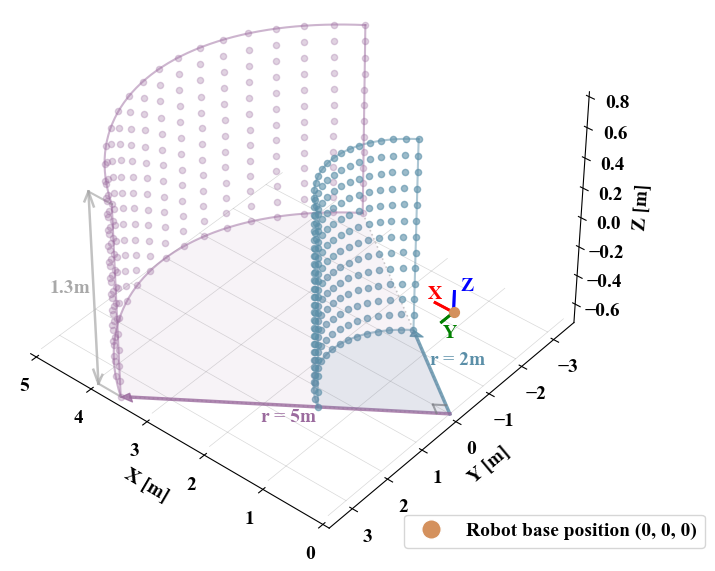
\includegraphics[width=0.9\columnwidth]{figure/adaptive_radius_3d.png}
    \caption{Illustration of the adaptive perception radius mechanism. The vertical distance map is constructed on a cylindrical sector with a fixed number of cells ($17 \times 13$). A smaller radius (blue) provides higher spatial resolution for precise near-field sensing, while a larger radius (purple) extends the perception range at the cost of reduced resolution. 
    The policy learns to dynamically adjust this radius based on the robot's locomotion state.}
    \label{fig:adaptive_radius}
\end{figure}

The critic operates on a privileged observation space to facilitate accurate estimation of the value function $V_t$. In addition to the actor's input vector $o_t$, the critic receives the noise-free ground-truth elevation map $\hat{\mathbf{E}}_t$ directly acquired from the simulation engine.
All components are then scaled, flattened and concatenated into a 648-dimensional vector to serve as input to the recurrent policy.

\subsubsection{Action Space}
The policy produces a composite action $\mu_t \in \mathbb{R}^{13}$ for each step at $50$ Hz to simultaneously handle motor control and perceptual modulation. 
The composite action $a_t$ is thus formally defined as
\begin{equation}
    a_t = \{q_t, r_t\}
    \label{eqn:action_vector}
\end{equation}
The specific components in (\ref{eqn:action_vector}) are:
\begin{itemize}
    \item \textit{Joint Targets:} The first 12 elements of $\mu_t$ specify target joint positions. They are scaled and superimposed onto a nominal configuration $q_{\text{default}}$ to yield the action targets $q_t \in \mathbb{R}^{12}$ defined as
    \begin{equation}
        q_t = s_a \cdot \mu_{t, 1:12} + q_{\text{default}}
    \end{equation}
    where $s_a$ is the action scale. 
    These targets are then executed by a low-level Proportional-Derivative (PD) controller.
    \item \textit{Adaptive Perception Radius:} The final element of $\mu_t$ dictates the perception radius $r_t \in [1, 5]$\,m for the subsequent timestep, which is directly used to shape the exteroceptive map based on current locomotion dynamics. 
    This range is empirically determined: a radius below 1\,m provides insufficient lookahead for timely obstacle avoidance maneuvers, whereas a radius exceeding 5\,m introduces excessive distal noise that degrades traversability estimation. Both extremes severely impair collision avoidance performance.
    % This structure establishes a feedback loop wherein the policy proactively shapes its future exteroceptive maps based on current locomotion dynamics.
\end{itemize}

\subsubsection{Reward Functions}
The reward function $\mathcal{R}$ integrates multiple objectives to encourage robust and efficient locomotion adhering to safety constraints. The total reward $r_t = \sum_i w_i r_i(t)$ is a weighted sum of the following components:

\begin{itemize}
    \item \textit{Motion Control:} Precise velocity tracking, postural stability, and energy efficiency are promoted by penalizing deviations in base orientation, excessive joint velocities or accelerations, and high-frequency action oscillations.
    
    \item \textit{Safety Mechanisms:} Safe and prolonged operation is ensured by penalizing critical failures such as body collisions, mesh interpenetrations, and joint limit violations. Furthermore, survival bonuses and foot air-time rewards are provided to foster dynamic and robust obstacle clearance.
    
    \item \textit{Active Perception:} The active sensing behavior is optimized by dynamically adapting the perception radius based on the robot's velocity and proximity to obstacles. Additional penalties on abrupt variations and boundary saturations ensure smooth and stable sensor adjustments.
\end{itemize}

\subsubsection{Terrain Design}
\textit{BarrierTrack} (Fig.~\ref{fig:terrain}), a customized environment assembling discrete obstacle modules, is designed to cultivate versatile locomotion. Each episode features a sequence of five obstacles of the same terrain type with progressively increasing difficulty according to a curriculum schedule. 

A curriculum-based strategy is adopted where each terrain type $\tau$ is parameterized by a difficulty scalar $s \in [0, 1]$, and its generation parameters are interpolated as $\mathbf{p}_\tau(s) = (1-s)\,\mathbf{p}_\tau^{\min} + s\,\mathbf{p}_\tau^{\max}$ based on Table~\ref{tab:terrain_params}. Perlin noise is superimposed onto ground surfaces to simulate terrain irregularity and prevent overfitting.


\begin{figure}[t]
    \centering
    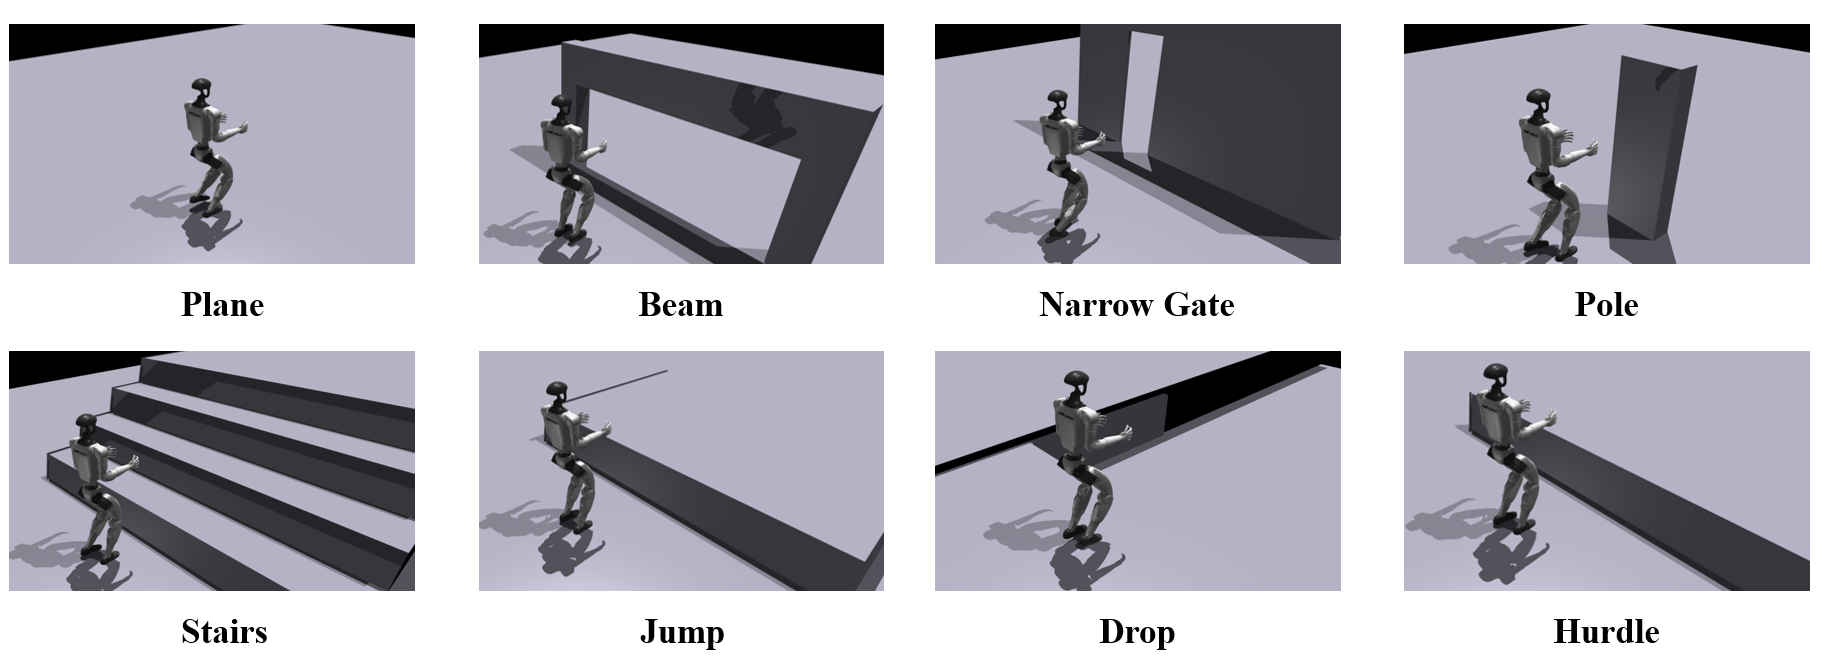
\includegraphics[width=\columnwidth]{figure/terrain.png}
    \caption{Examples of procedurally generated obstacles in our \textit{BarrierTrack} training environment. The curriculum includes a diverse set of challenges such as stairs, drop, hurdles, and constrained passages like beams and narrow gates, promoting the development of a versatile locomotion policy.}
    \label{fig:terrain}
\end{figure}

\begin{table}[h]
\vspace{3pt}
\centering
\caption{Parameters for generating curriculum training terrains. The $\uparrow$ symbol indicates the parameter value increases as difficulty scales up ($\mathbf{p}_\tau^{\min} < \mathbf{p}_\tau^{\max}$), while the $\downarrow$ symbol indicates the value decreases as the task becomes harder ($\mathbf{p}_\tau^{\min} > \mathbf{p}_\tau^{\max}$).}
\label{tab:terrain_params}
\setlength{\tabcolsep}{4pt}
\begin{tabular}{@{}llcc@{}}
\toprule
\textbf{Terrain} & \textbf{Param. (m)} & $\mathbf{p}_\tau^{\min}$ & $\mathbf{p}_\tau^{\max}$ \\
\midrule
\multirow{2}{*}{\textbf{Beam}} & Clearance Height $\downarrow$ & 1.33 & 1.10 \\
& Beam Depth $\uparrow$ & 0.20 & 0.20 \\
\addlinespace
\multirow{2}{*}{\textbf{Narrow Gate}} & Gate Width $\downarrow$ & 0.80 & 0.45 \\
& Position Offset $\uparrow$ & 0.00 & 0.60 \\
\addlinespace
\multirow{2}{*}{\textbf{Pole}} & Pole Width $\downarrow$ & 0.50 & 0.10 \\
& Position Offset $\uparrow$ & 0.00 & 0.00 \\
\addlinespace
\multirow{2}{*}{\textbf{Stairs}} & Step Height $\uparrow$ & 0.10 & 0.30 \\
& Step Length $\downarrow$ & 0.50 & 0.30 \\
\addlinespace
\multirow{2}{*}{\textbf{Jump}} & Wall Height $\uparrow$ & 0.05 & 0.40 \\
& Wall Depth $\uparrow$ & 0.10 & 0.30 \\
\addlinespace
\multirow{2}{*}{\textbf{Drop}} & Drop Height $\uparrow$ & 0.10 & 0.60 \\
& Platform Length $\downarrow$ & 0.50 & 0.30 \\
\addlinespace
\multirow{2}{*}{\textbf{Hurdle}} & Hurdle Height $\uparrow$ & 0.05 & 0.40 \\
& Hurdle Depth $\uparrow$ & 0.05 & 0.10 \\
\bottomrule
\end{tabular}
\end{table}

\subsection{Training Architecture}
\label{sec:training_architecture}

As shown in Fig.~\ref{fig:network_architecture}, the training framework employs an asymmetric recurrent actor-critic architecture with a Gated Recurrent Unit (GRU) to capture short-horizon temporal dependencies during locomotion. This framework allows the critic to leverage privileged simulation states to accelerate convergence. 
The critic combines the recurrent states with noise-free ground truth including elevation to enable precise value estimation. 
In contrast, the actor operates exclusively on deployable observations.
% This asymmetry facilitates robust policy learning while ensuring the actor remains deployable under real-world sensor limitations.
The policy is optimized using the Proximal Policy Optimization (PPO) algorithm. Note that the observation vector $o_t$ is processed through two separate MLP encoders, which independently encode the exteroceptive inputs $\mathbf{E}_t$ and $\mathbf{D}_t$ into 32-dimensional latent variables. These latent representations are concatenated to form a 64-dimensional environmental embedding and fused with the proprioceptive states before being passed to the actor and critic heads.

A distinguishing feature of the proposed architecture is the closed-loop modulation of perceptual parameters. Conditioned on the recurrent hidden state, the actor outputs the perception radius $r_t$ to tightly couple the sensing range with robot states and obstacle proximity.
% to effectively treat perception as an actuated degree of freedom.